\setcounter{equation}{0}

Факты ниже перекликаются с разделом~<<\nameref{varcoef-topic-anchor}>>. Можно перейти сразу к теме вопроса:~<<\nameref{constcoef-equation-anchor}>>.

\Def Вектор-функции $\vec{y}_1(x), \ldots , \vec{y}_k(x)$, определённые на промежутке $I$, называются линейно зависимыми, если
$$\exists \alpha_1, \ldots , \alpha_k \in \mathbb{R} : 
\Big( \sum\limits_{i=1}^k \alpha_i^2 \neq 0 \wedge \sum\limits_{i=1}^k \alpha_i\vec{y}_i(x) \equiv \vec{0} \Big)$$

на всем $I$.

\Def Пусть $\vec{y}_1(\vec{x}), \ldots , \vec{y}_n(\vec{x})$ -- вектор-функции с $n$ компонентами. Функция
$$W(x) = 
\begin{vmatrix}
  y_1^1(x)& y_2^1(x)& \ldots& y_n^1(x)\\
  \vdots& \vdots& \ddots& \vdots\\
  y_1^n(x)& y_2^n(x)& \ldots& y_n^n(x)
\end{vmatrix}$$

называется определителем Вронского (вронскианом) для заданных вектор-функций.

\Lemma Если вронскиан системы $\vec{y}_1(x), \ldots , \vec{y}_n(x)$ отличен от нуля хотя бы в одной
точке, то все эти функции линейно независимы.

\Proof
Пусть эти функции линейно зависимы, тогда векторы $\vec{y}_1(x_0), \ldots , \vec{y}_n(x_0)$ линейно зависимы в каждой точке $x_0$, а значит, определитель матрицы, составленной из векторов (то есть, значение вронскиана в точке $x_0$), равен нулю.
\EndProof

\Lemma Если вектор-функции $\vec{y}_1(x), \ldots , \vec{y}_n(x)$ -- решения некоторой системы линейных однородных уравнений на промежутке $I$ и $\exists x_0 \in I: W(x_0) = 0$, то $\vec{y}_1(x), \ldots , \vec{y}_n(x)$ линейно зависимы на $I$.

\Proof
$\vec{y'} = A(x)(\vec{y})$

В точке $x_0$ векторы $\vec{y}_1(x), \ldots, \vec{y}_n(x)$ линейно зависимы, значит, существует их линейная комбинация, которая обращается в ноль в точке $x_0 : \sum\limits_{i=1}^nc_i\vec{y}_i(x_0) \equiv \vec{0}$.

Рассмотрим $n$ задач Коши для $\vec{y}(x_0) = \vec{y}_k(x_0)$. Рассмотрим функцию $\vec{y}(x) = \sum\limits_{i=1}^nc_i\vec{y}_i(x)$ на $I$. 

$\vec{y}(x_0) = \vec{0} \Rightarrow$ по теореме о существовании и единственности $\vec{y}(x) = \sum\limits_{i=1}^nc_i\vec{y}_i(x) \equiv \vec{0}$
\EndProof

\Def Фундаментальная система решений (ФСР) для СЛДУ (СЛДУ определена в пункте 4.3) -- набор $n$ линейно независимых решений системы (здесь $n$ -- кол-во уравнений).

\Lemma  Для любой СЛДУ существует ФСР.

\Proof Пусть $x_0 \in [a, b], \text{и} (\vec{y}_0)_1, \ldots , (\vec{y}_0)_n$ -- числовые линейно независимые векторы. Составим систему задач Коши:

\begin{equation*}
    \begin{cases}
        \vec{y'} = A(x)\vec{y}&\\
        \vec{y}(x_0) = \vec{y}_0 &
    \end{cases}
\end{equation*}

Пусть $\vec{z}_1, \ldots , \vec{z}_n$ -- решения этих задач, тогда их вронскиан равен определителю матрицы,
составленной из $(\vec{y}_0)_i$, следовательно, он не равен нулю, и ФСР существует.

\EndProof

\Lemma Любое решение СЛДУ единственным образом представимо в виде линейной комбинации векторов ФСР.

\Proof Пусть $x_0 \in [a, b], \vec{y} - \text{решение системы, и } \vec{y}_1, \ldots , \vec{y}_n$ -- ФСР, тогда
$\vec{y}_1(x_0), \ldots , \vec{y}_n(x_0)$ линейно независимы, и $\vec{y}(x_0)$ единственным образом выражается через
них. В силу единственности решения задачи Коши коэффициенты линейной комбинации
окажутся одними и теми же для всех точек отрезка.

\EndProof

\paragraph{Линейные однородные ДУ $n$-го порядка с постоянными коэффициентами}
\label{constcoef-equation-anchor}

\begin{equation}\label{varcoef-4}
    L(y) = a_0y^{(n)} + a_1y^{(n-1)} +\ldots + a_{n-1}y' + a_ny = 0
\end{equation}

$(a_i \in \mathbb{R}, a_0 \neq 0, y : \mathbb{R} \to \mathbb{R})$
Существование и единственность решения следуют из таковых для системы

\begin{equation*}
    \begin{cases}
        \vec{y}_1' = y' = y_2&\\
        \vec{y}_2' = y'' = y_3&\\
        \ldots&\\
        \vec{y}_{n-1}' = y_n&\\
        \vec{y}_n' = \frac{1}{a_0}(- a_ny_1 - a_{n-1}y_2 - \ldots - a_1y_n)
    \end{cases}
\end{equation*}

(здесь $y_1 = y$)

Для уравнения \ref{varcoef-4} можно определить вронскиан, равный вронскиану написанной выше системы.

Найдём решение системы \ref{varcoef-4} в виде $y = e^{\lambda x}$:

$$M(\lambda) = a_0\lambda^n + \ldots + a_{n-1}\lambda + a_n$$
$$L(e^{\lambda x}) = M(\lambda)e^{\lambda x} = 0$$

Поскольку экспонента никогда не обнуляется (даже в поле комплексных чисел), то единственный возможный вариант -- это $M(\lambda) = 0$. Уравнение $M(\lambda) = 0$ называется характеристическим, как и многочлен в его левой части.

\Statement Пусть $\lambda_1, \ldots, \lambda_n$ -- однократные корни $M(\lambda)$, тогда решения $y_i = e^{\lambda_ix}$ линейно независимы.

\Proof
\begin{center}
    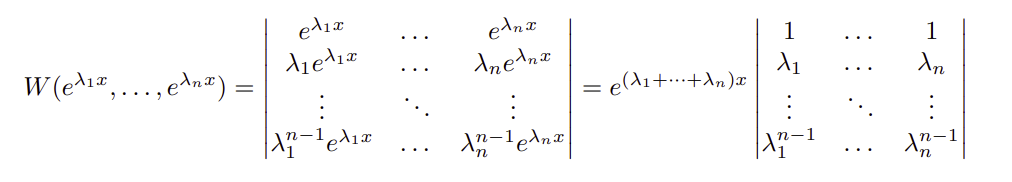
\includegraphics[width=0.9\linewidth]{images/vandermond.png}
\end{center}
Получившийся \textit{определитель Вандермонда} не будет равен нулю в силу того, что все $\lambda_i$ различны.


Если все $a_i \in \mathbb{R}$, то все комплексные корни $M(\lambda)$ разбиваются на пары сопряжённых
между собой комплексных чисел. Мнимая и действительная части решений, соответствующих таким корням, сами являются решениями:
$$\lambda = \alpha + i\beta, \overline{\lambda} = \alpha - i\beta$$
$$y_1 = e^{\lambda x}$$
$$\overline{y}_1 = e^{\overline{\lambda} x}$$
$$z_1 = \frac{y_1 + \overline{y_1}}{2} = e^{\alpha x} cos\beta x$$
$$z_2 = \frac{y_1 - \overline{y_1}}{2} = e^{\alpha x} sin\beta x$$

Замена $y_1$ и $\overline{y}_1$ на $z_1$ и $z_2$ является корректным переходом в другой базис (проверяется построением матрицы перехода и подсчётом определителя), а потому линейная оболочка не изменится.
\EndProof

\Statement Пусть $\lambda$ -- корень $M(\lambda)$ кратности $\ell$, тогда функции $e^{\lambda x}, xe^{\lambda x}, \ldots, x^{\ell-1}e^{\lambda x}$
 являются решениями \ref{varcoef-4}.
 
\Lemma Пусть $y = x^se^{\lambda x}$, где $\lambda$ -- корень характеристического уравнения кратности $\ell$,
тогда

$$L(x^se^{\lambda x}) =
\begin{cases}
    0,& s < \ell\\
    (b_0x^{s-\ell} + b_1x^{s-\ell -1} +  \ldots + b_{s-\ell} )e^{\lambda x},& s \geq \ell
\end{cases}
$$

\Proof
Пусть $z$ и $\lambda$ -- комплексные числа; сначала докажем, что

$\Big( (e^{\lambda z})_{\lambda}^{(s)} \Big)_z^{(p)} = \Big( (e^{\lambda z})_{z}^{(p)} \Big)_{\lambda}^{(s)}$, или же $(z^se^{\lambda z})_z^{(p)} = (\lambda^pe^{\lambda z})_{\lambda}^{(s)}$

Рассмотрим некую формальную операцию $\cdot'_x (\cdot'_{\lambda})$, для которой верны следующие соотношения:

$$(x^s)'_x = sx^{s-1}$$
$$(a)'_x = 0$$
$$(e^{\lambda x})'_x = \lambda e^{\lambda x}$$
$$(\alpha f_1 + \beta f_2)'_x = \alpha(f_1)'_x + \beta(f_2)'_x$$
$$(f_1 \cdot f_2)'_x = (f_1)'_x \cdot f_2 + f_1 \cdot (f_2)'_x$$

Теперь докажем наше утверждение:

$((z^s e^{\lambda z})_z^{(p)}) = \sum\limits_{k=1}^p C_p^k (z^s)_z^{(k)} (e^{\lambda z})_z^{(p-k)}$

$ = \sum\limits_{k=0}^pC_p^ks(s-1)\ldots(s-(k-1))z^{s-k}\lambda^{p-k}e^{\lambda z}$

$= \sum\limits_{k=0}^{min(p, s)}C_p^kC_s^kk!z^{s-k}\lambda^{p-k}e^{\lambda z}$

Заметим, что $(\lambda^pe^{\lambda z})_{\lambda}^{(s)}$ раскроется в такое же выражение ввиду <<структурной симметрии>>.

Найдем: $L(x^s e^{\lambda x}) = a_0(x^s e^{\lambda x})_x^{(n)} + a_1(x^s e^{\lambda x})_x^{(n-1)} + \ldots + a_n(x^s e^{\lambda x})$

$= a_0\Big((e^{\lambda x})_{\lambda}^{(s)}\Big)_x^{(n)} + a_1\Big((e^{\lambda x})_{\lambda}^{(s)}\Big)_x^{(n-1)} + \ldots + a_n\Big((e^{\lambda x})_{\lambda}^{(s)}\Big)$

$= a_0\Big((e^{\lambda x})_x^{(n)}\Big)_{\lambda}^{(s)} + a_1\Big((e^{\lambda x})_x^{(n-1)}\Big)_{\lambda}^{(s)} + \ldots + a_n\Big((e^{\lambda x})\Big)_{\lambda}^{(s)}$

$= \Big(a_0(e^{\lambda x})_x^{(n)} + a_1(e^{\lambda x})_x^{(n-1)} + \ldots + a_n(e^{\lambda x}) \Big)_{\lambda}^{(s)}$

$= \Big(e^{\lambda x}M(\lambda) \Big)_{\lambda}^{(s)} = \sum\limits_{k=0}^sC_s^k(M(\lambda))_{\lambda}^{(k)}(e^{\lambda x})_{\lambda}^{(s-k)}$

$= \sum\limits_{k=\ell}^sC_s^k(M(\lambda))_{\lambda}^{(k)}(e^{\lambda x})_{\lambda}^{(s-k)}$

Следовательно, $b_i = C_s^k(M(\lambda))_{\lambda}^{(k)}$, и лемма доказана.

Исходное утверждение выводится из леммы применением того факта, что корень кратности $s$ многочлена $P(x)$ является корнем $P, P', \ldots, P^{(s-1)}$
\EndProof


\Def Квазимногочлен — произведение многочлена на экспоненту с линейной
функцией в показателе.

\Statement $(P_m(x)e^{\lambda x})'_x = Q_m(x)e^{\lambda x}$

\Th (О структуре ФСР)

Пусть $\lambda_1, \ldots, \lambda_k$ корни характеристического многочлена ($M(\lambda)$) кратности $l_1, \ldots, l_k$. Тогда набор функций $x^s e^{\lambda_i x}$, где $s = 0, \ldots, l_1-1$, $i = 1, \ldots, k$ является ФСР для уравнения \ref{varcoef-4}

\Proof
Докажем от противного. Пусть ЛЗ, то есть 
\[ \exists {c_i} (\sum_{}^{} c_i^2 \neq 0)\hookrightarrow \sum_{i=1}^{n} c_i y_i(x) = 0\]

Сгруппируем слагаемые при одинаковых $e^{\lambda_i x}$: $\sum_{i=1}^{k} e^{\lambda_i x} p^i(x) = 0$. Значит, хотя бы один из многочленов $p^i(x) \neq 0$. Без ограничения общности примем $p^1(x) \neq 0$, домножим равенство на $e^{-\lambda_k x}$:
\[e^{x(\lambda_1 - \lambda_k)} p^1(x) +
e^{x(\lambda_2 - \lambda_k)} p^2(x) + ... + 
e^{x(\lambda_{k-1} - \lambda_k)} p^{k-1}(x) + p^k(x) = 0\]
Воспользуемся допущением и продифференцируем $l_k$ раз~--- до того пока не уйдет $p^k(x)$
\[e^{x(\lambda_1 - \lambda_k)} Q^1(x) +
e^{x(\lambda_2 - \lambda_k)} Q^2(x) + ... + 
e^{x(\lambda_{k-1} - \lambda_k)} Q^{k-1}(x) = 0\]
Заметим, что $(\lambda_i - \lambda_k)x - (\lambda_{k-1} - \lambda_k)x = (\lambda_i - \lambda_{k-1})x$. Дифференцируем и доходим до 
\[e^{x(\lambda_1 - \lambda_2)} R(x) = 0,\] откуда $R(x) = 0$, но тогда $p^1(x) = 0$. Противоречие
\EndProof
